\section{Hiện thực bảo mật hệ thống}
\subsection{Hiện thực giảm thiểu bề mặt tấn công}
Để giảm thiểu việc tấn công bề mặt cho hệ thống Yocto, không thể chỉ dừng lại ở việc cấu hình hệ thống mà còn bao gồm việc kiểm soát chặt chẽ các thiết lập mặc định và thành phần của hệ thống. Khi tạo một dự án mới, mặc định là hệ thống sẽ cung cấp một file local.conf ban đầu bao gồm các tính năng như cho phép mật khẩu rỗng hoặc đăng nhập root trực tiếp bằng cách sử dụng biến \texttt{EXTRA\_IMAGE\_FEATURES} với dòng lệnh:

\begin{figure}[!h]
    \centering
    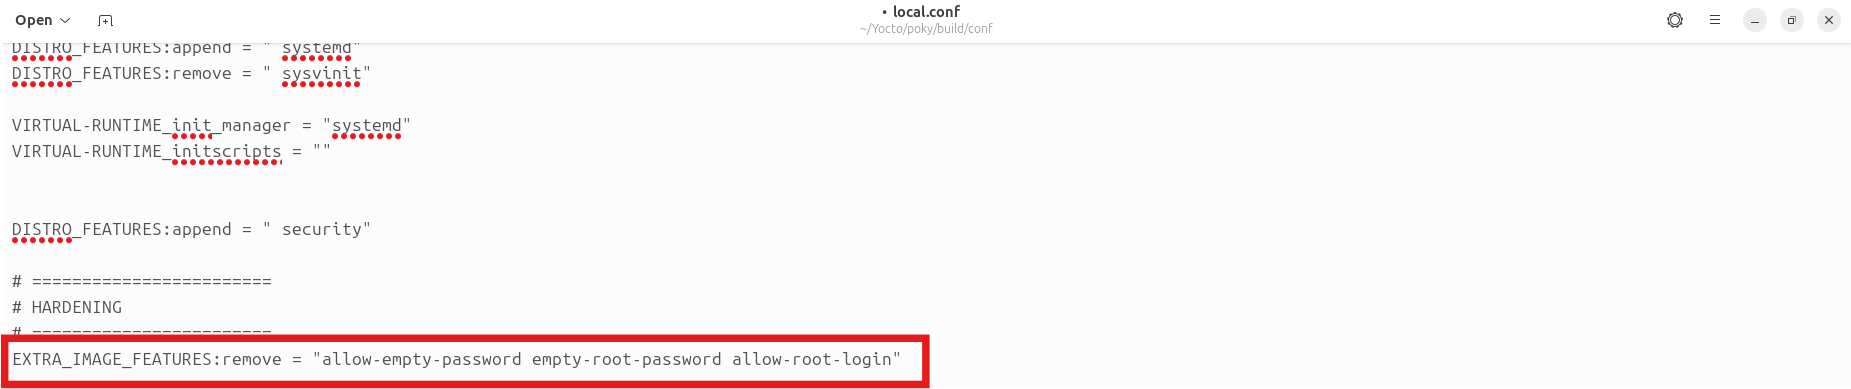
\includegraphics[width=1\textwidth]{image/gtbm.png}
    \caption{Giảm thiểu bề mặt tấn công trong Yocto Project}
    \label{fig:gtbm} 

\end{figure}

Để đảm bảo an toàn cho hệ thống, các lựa chọn “allow\-empty-password”, “allow\-root\-login” hoặc “empty\-root\-password” cần đảm bảo không phải là một trong những \texttt{IMAGE\_FEATURES}. 
Ngoài ra, chỉ giữ lại các thành phần thực sự cần thiết cho hệ thống Yocto thông qua các biến cấu hình như \texttt{DISTRO\_FEATURES} và  \texttt{IMAGE\_FEATURES}, nhằm giảm thiểu bề mặt tấn công. Bên cạnh đó, cần xem xét và tinh chỉnh cấu hình nhân hệ điều hành để đảm bảo chỉ bao gồm các trình điều khiển và tính năng cần thiết, tránh đưa vào những thành phần dư thừa có thể gây rủi ro bảo mật thông qua việc tùy chỉnh các thành phần trong kernel như \texttt{CONFIG\_DEVMEM} và \texttt{STRICT\_DEVMEM} nhằm hạn chế khả năng truy cập trực tiếp vào bộ nhớ thiết bị từ không gian người dùng. Điều này góp phần ngăn chặn các hành vi khai thác ở mức thấp, từ đó nâng cao mức độ an toàn tổng thể của hệ thống.

Một biện pháp quan trọng khác nhằm giảm thiểu rủi ro bị tấn công bề mặt là hạn chế hoặc không cho phép người dùng cài đặt thêm phần mềm sau khi thiết bị đã được triển khai. Trong các hệ thống sử dụng Yocto, phần mềm thường được build sẵn vào image, và hệ thống không được thiết kế như các bản phân phối Linux thông thường với trình quản lý gói mở cho người dùng. Việc cho phép cài đặt thêm package có thể làm mất kiểm soát cấu hình hệ thống, dẫn đến nguy cơ xuất hiện các phần mềm không được kiểm chứng hoặc chứa lỗ hổng bảo mật. Để giảm thiểu các rủi ro này, các developer không sử dụng các định dạng package như ipk, rpm hoặc deb trong quá trình build, đồng thời loại bỏ các thành phần package manager khỏi image. Ngoài ra, việc loại bỏ feature package-management và thiết lập hệ thống file ở chế độ chỉ đọc (read-only root filesystem) sẽ giúp ngăn chặn việc cài đặt hoặc thay đổi phần mềm trong quá trình vận hành.
Việc tinh chỉnh cấu hình kernel, loại bỏ các driver và tính năng không cần thiết, cũng như kích hoạt các tùy chọn bảo mật, giúp hạn chế khả năng khai thác từ các lỗ hổng mức thấp. Những biện pháp này góp phần xây dựng một hệ thống an toàn, ổn định và phù hợp với môi trường nhúng.



\subsection{Hiện thực Selinux}

Nhóm thực hiện bổ sung layer meta-selinux vào môi trường build:
\medskip

\begin{figure}[!h]
\renewcommand*\DTstyle{\ttfamily}
\dirtree{%
.1 meta-selinux/.
.2 classes/.
.2 conf/.
.2 recipes-core/.
.2 recipes-kernel/.
.2 recipes-security/.
.3 refpolicy/.
.3 selinux/.
.3 packagegroups/.
.3 images/.
.2 recipes-support/.
}
\caption{Cấu trúc thư mục chính của layer meta-selinux}
\label{fig:meta-selinux-structure}
\end{figure}
Hình \ref{fig:meta-selinux-structure} mô tả cấu trúc thư mục chính của layer \texttt{meta-selinux} trong Yocto Project. Layer này cung cấp các thành phần cần thiết để tích hợp cơ chế bảo mật SELinux vào hệ thống Linux nhúng. Trong đó, thư mục \texttt{classes} chứa các lớp hỗ trợ quá trình build và cấu hình SELinux; thư mục \texttt{conf} lưu trữ các thiết lập cấu hình của layer. Các thư mục \texttt{recipes-core}, \texttt{recipes-kernel} và \texttt{recipes-support} chứa các recipe bổ sung hoặc chỉnh sửa cho các thành phần hệ thống liên quan đến SELinux.

Đặc biệt, thư mục \texttt{recipes-security} đóng vai trò trung tâm trong việc triển khai cơ chế bảo mật. Bên trong thư mục này, \texttt{refpolicy} chứa các policy chuẩn của SELinux, \texttt{selinux} cung cấp các gói và công cụ hỗ trợ SELinux, \texttt{packagegroups} định nghĩa các nhóm package cần thiết, trong khi \texttt{images} hỗ trợ tích hợp SELinux trực tiếp vào image được build. Cấu trúc phân lớp này giúp việc quản lý, mở rộng và tùy chỉnh chính sách bảo mật trở nên linh hoạt và thuận tiện hơn trong quá trình phát triển hệ thống nhúng sử dụng Yocto Project.

SELinux hỗ trợ nhiều loại policy khác nhau nhằm đáp ứng các yêu cầu bảo mật và mức độ kiểm soát truy cập khác nhau của hệ thống. Trong đó, hai policy phổ biến nhất là \texttt{refpolicy-targeted} và \texttt{refpolicy-mls}. Mỗi policy được thiết kế cho các mục đích sử dụng riêng, từ các hệ thống Linux thông thường đến các môi trường yêu cầu bảo mật nghiêm ngặt. Việc lựa chọn policy phù hợp có ảnh hưởng trực tiếp đến mức độ bảo vệ, hiệu năng và độ phức tạp trong quá trình quản trị hệ thống.

\begin{table}[H]
\centering
\caption{So sánh các policy phổ biến của SELinux}
\label{tab:selinux-policy-comparison}

\renewcommand{\arraystretch}{1.4}

\begin{tabular}{|p{4cm}|p{3.5cm}|p{3cm}|p{4cm}|}
\hline
\textbf{Policy} & \textbf{Đặc điểm} & \textbf{Mức độ bảo mật} & \textbf{Trường hợp sử dụng} \\ \hline

\texttt{refpolicy-targeted}
&
Chỉ áp dụng cơ chế kiểm soát truy cập cho các tiến trình và dịch vụ quan trọng
&
Trung bình đến cao
&
Hệ thống nhúng, máy chủ thông thường, môi trường cần cân bằng giữa bảo mật và hiệu năng
\\ \hline

\texttt{refpolicy-mls}
&
Áp dụng cơ chế Multi-Level Security (MLS), kiểm soát truy cập theo nhiều cấp độ bảo mật
&
Rất cao
&
Hệ thống quân sự, chính phủ hoặc các môi trường yêu cầu phân cấp dữ liệu nghiêm ngặt
\\ \hline

\texttt{minimum}
&
Policy tối giản với số lượng rule hạn chế, chỉ bảo vệ các thành phần cơ bản
&
Cơ bản
&
Hệ thống tài nguyên hạn chế hoặc môi trường thử nghiệm
\\ \hline

\end{tabular}
\end{table}

Trong phạm vi đề tài, policy \texttt{refpolicy-targeted} được lựa chọn để triển khai trên hệ thống Yocto Linux. Nguyên nhân là do policy này cung cấp mức độ bảo mật phù hợp cho các hệ thống nhúng IoT nhưng vẫn đảm bảo tính ổn định và hiệu năng của hệ thống. So với \texttt{refpolicy-mls}, policy \texttt{targeted} có cấu hình đơn giản hơn, ít tiêu tốn tài nguyên và dễ triển khai trong môi trường thiết bị nhúng có giới hạn về bộ nhớ và năng lực xử lý. Đồng thời, policy này vẫn đủ khả năng bảo vệ các dịch vụ quan trọng khỏi các hành vi truy cập trái phép hoặc leo thang đặc quyền trong quá trình vận hành hệ thống.

Để tích hợp SELinux vào hệ thống Yocto, trước tiên cần bổ sung layer \texttt{meta-selinux} vào danh sách layer trong file \texttt{bblayers.conf}. Layer này cung cấp các recipe, policy và công cụ cần thiết để hỗ trợ cơ chế Mandatory Access Control (MAC) trên hệ thống Linux nhúng. Đồng thời, do \texttt{meta-selinux} phụ thuộc vào các layer từ repository \texttt{meta-openembedded}, bao gồm \texttt{meta-oe} và \texttt{meta-python}, các layer này cũng cần được thêm vào môi trường build để đảm bảo đầy đủ thư viện và thành phần hỗ trợ liên quan.

Sau khi thêm layer, hệ thống được cấu hình để kích hoạt SELinux thông qua việc bổ sung \texttt{selinux} vào biến \texttt{DISTRO\_FEATURES} trong file \texttt{local.conf}. Việc này giúp Yocto tự động tích hợp các thành phần SELinux vào image trong quá trình build. Ngoài ra, các package phụ trợ như \texttt{acl}, \texttt{xattr} và \texttt{pam} cũng được thêm vào nhằm đảm bảo SELinux có đầy đủ cơ chế quản lý quyền truy cập, extended attributes và xác thực người dùng.

\begin{figure}[!h]
    \centering
    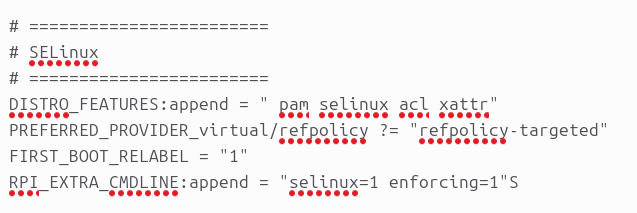
\includegraphics[width=0.7\textwidth]{image/selinuxx.png}
    \caption{Selinux}
    \label{fig:selinux} 
\end{figure}

Tiếp theo, hệ thống cần lựa chọn chính sách bảo mật phù hợp thông qua biến \texttt{PREFERRED\_}\\
\texttt{PROVIDER\_virtual/refpolicy} sử dụng policy \texttt{refpolicy-targeted}.


Sau khi hoàn tất các bước cấu hình, hệ thống được build lại để tạo ra image tích hợp SELinux. Trong quá trình vận hành, SELinux có thể hoạt động ở ba chế độ chính: enforcing, permissive và disabled. Ở chế độ enforcing, SELinux thực thi nghiêm ngặt các chính sách bảo mật, mọi hành vi truy cập không được phép sẽ bị chặn. Ở chế độ permissive, hệ thống không chặn các hành vi vi phạm mà chỉ ghi lại nhật ký, giúp nhà phát triển theo dõi và điều chỉnh chính sách phù hợp trong giai đoạn kiểm thử. Trong khi đó, chế độ disabled sẽ vô hiệu hóa hoàn toàn SELinux, hệ thống quay về cơ chế phân quyền truyền thống.
Việc kiểm tra trạng thái hoạt động của SELinux có thể được thực hiện thông qua các công cụ như getenforce hoặc sestatus. Thông qua đó, có thể xác định chế độ hiện tại của SELinux và đánh giá hiệu quả của các chính sách bảo mật đã được áp dụng trong hệ thống.

\subsection{Hiện thực dm-verity}

Quá trình triển khai dm-verity nhằm bảo vệ tính toàn vẹn của hệ thống được thực hiện qua các giai đoạn từ xây dựng hình ảnh hệ thống (\textit{system image}) tại môi trường phát triển cho đến quá trình thực thi kiểm chứng tại thiết bị đích. Cụ thể:

\subsubsection{Giai đoạn tiền xử lý và tách phân vùng dữ liệu}

Tiến trình bắt đầu bằng việc xây dựng image hệ thống gốc được đóng gói dưới định dạng \texttt{.wic}. Từ image này, phân vùng \textit{rootfs} tương ứng với phân vùng \texttt{p2} được tách riêng biệt để làm dữ liệu đầu vào cho quá trình tạo dữ liệu (\textit{metadata}) của dm-verity. Đây là bước then chốt nhằm đảm bảo toàn bộ thông tin băm (\textit{hash}) được sinh ra từ chính xác nội dung cuối cùng của \textit{rootfs} sau khi biên dịch, tạo sự đồng nhất tuyệt đối giữa dữ liệu tính toán và dữ liệu thực tế trên thiết bị.

\subsubsection{Khởi tạo cấu trúc cây băm (Hash Tree) và xác thực metadata}

Sử dụng công cụ \texttt{veritysetup}, hệ thống tiến hành chia phân vùng \texttt{p2} thành các khối dữ liệu (\textit{blocks}) có kích thước cố định. Tại đây, mỗi khối dữ liệu được xử lý qua thuật toán băm SHA-256 để tạo ra các giá trị băm tương ứng. Các giá trị này được tổ chức theo cấu trúc cây băm nhiều mức (\textit{Merkle Tree}), dẫn đến hai thành phần đầu ra quan trọng:

\begin{itemize}
    \item \texttt{rootfs.hash}: tệp tin chứa toàn bộ cấu trúc cây băm của phân vùng.
    \begin{figure}[!h]
    \centering
    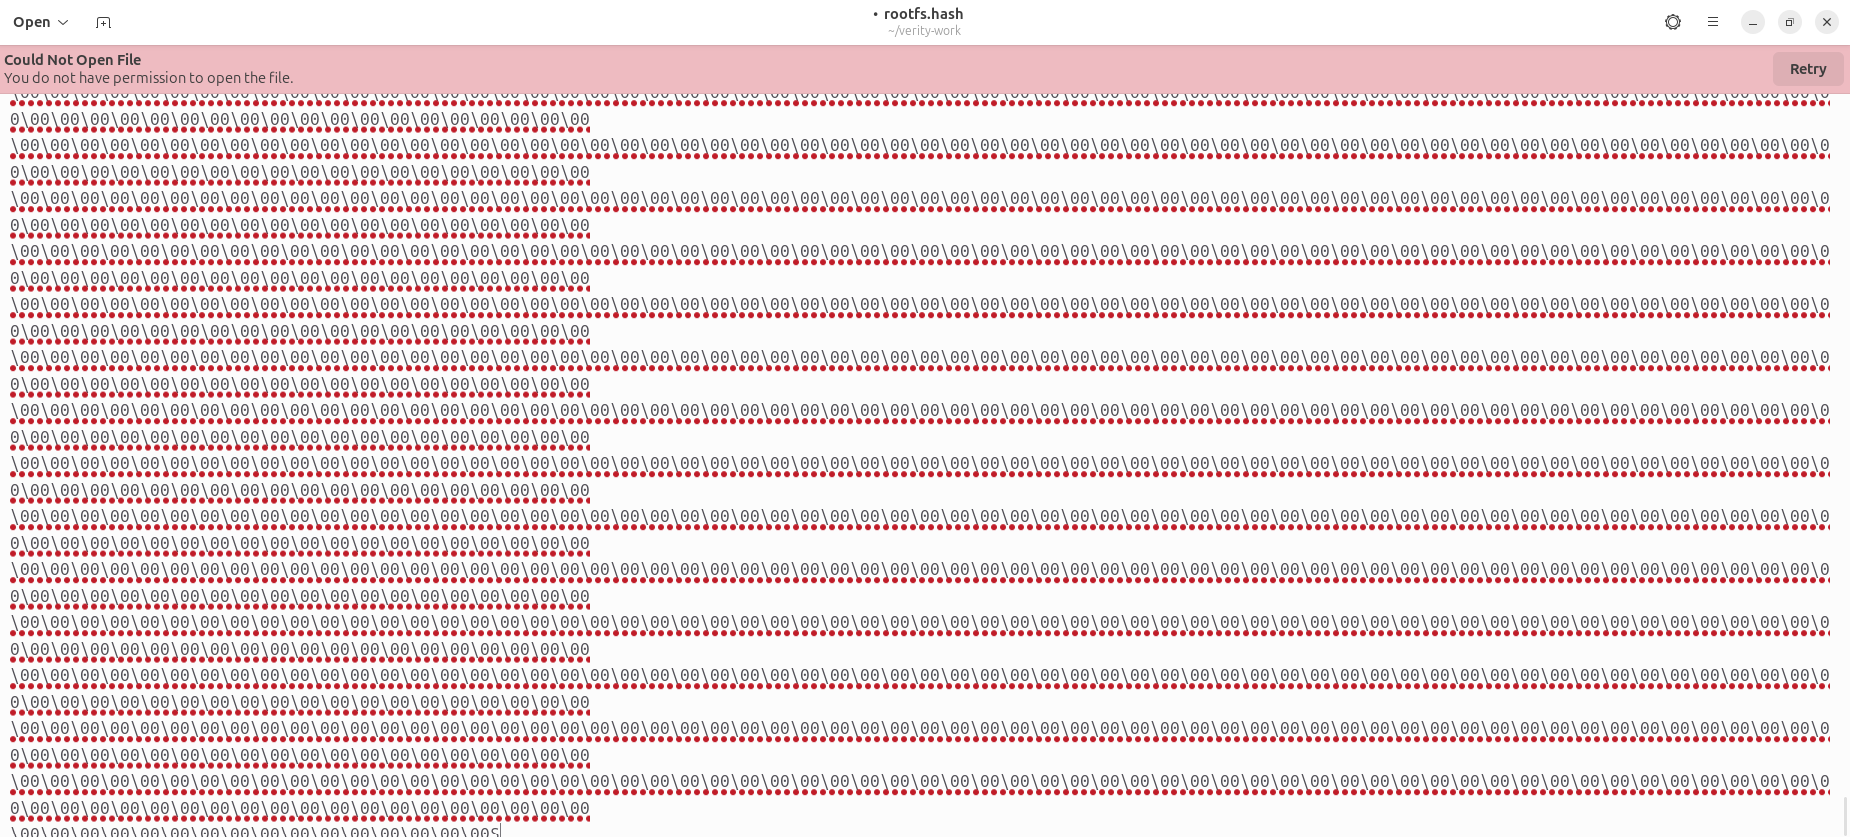
\includegraphics[width=1\textwidth]{image/roothash.png}
    \caption{Cấu trúc cây băm của rootfs}
    \label{fig:roothash} 
\end{figure}

    \item \texttt{root.hash}: giá trị băm gốc (\textit{root hash}), đại diện duy nhất cho tính toàn vẹn của toàn bộ phân vùng \textit{rootfs}.
\begin{figure}[!h]
    \centering
    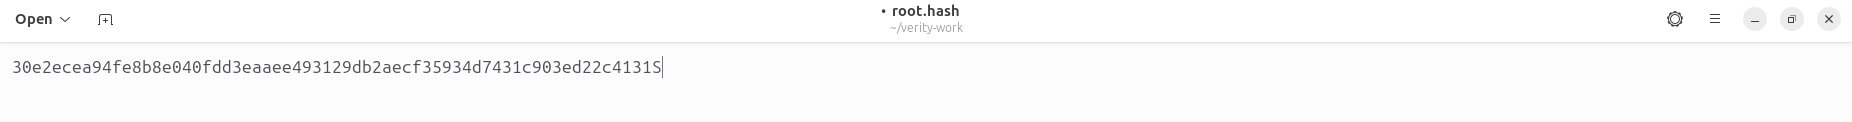
\includegraphics[width=1\textwidth]{image/root.png}
    \caption{Giá trị băm gốc (root hash)}
    \label{fig:rootkey} 
\end{figure}

  \end{itemize}

Để đảm bảo độ tin cậy, lệnh \texttt{veritysetup verify} được thực thi nhằm kiểm tra tính nhất quán giữa dữ liệu gốc và các thành phần \textit{metadata} vừa khởi tạo trước khi tiến hành nạp vào thiết bị.
\begin{figure}[!h]
    \centering
    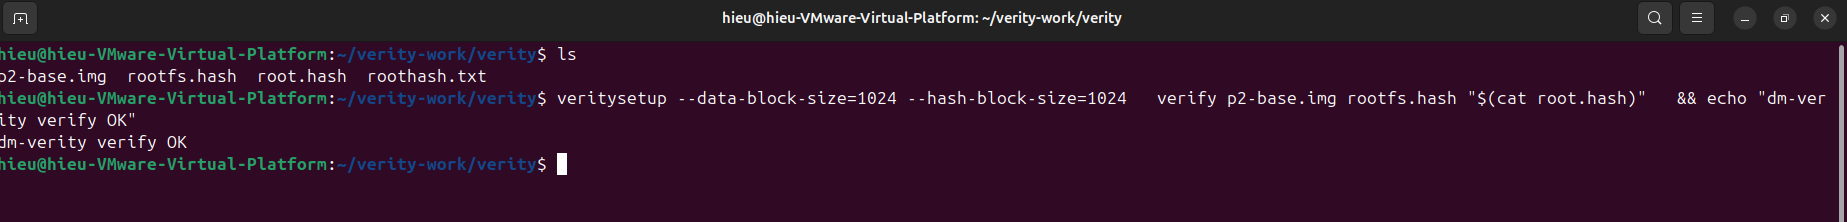
\includegraphics[width=1\textwidth]{image/verityok.png}
    \caption{Kết quả xác thực metadata của dm-verity}
    \label{fig:verityok} 
\end{figure}

\subsubsection{Triển khai và cấu hình giai đoạn khởi động sớm}

Sau khi xác thực thành công, hình ảnh hệ thống được nạp vào thẻ nhớ SD. Trong cấu trúc này, phân vùng \texttt{p1} đảm nhiệm vai trò khởi động (\textit{boot partition}), trong khi \texttt{p2} chứa \textit{rootfs} cần được bảo vệ. Các tệp tin \texttt{root.hash} và \texttt{rootfs.hash} được lưu trữ vào thư mục \texttt{/verity} trên phân vùng \texttt{p1}, cho phép hệ thống tệp trong bộ nhớ tạm (\textit{initramfs}) có thể truy xuất trong giai đoạn khởi động sớm.

\subsubsection{Cơ chế kiểm chứng thực thi tại thiết bị đích}

Tại thiết bị đích, tiến trình khởi động được điều khiển bởi Kernel và \textit{initramfs}. Tập lệnh \texttt{/init} trong \textit{initramfs} thực hiện gắn kết (\textit{mount}) phân vùng boot \texttt{p1}, truy xuất các tệp tin băm và sử dụng lệnh \texttt{veritysetup open} để thiết lập một thiết bị ánh xạ (\textit{mapping device}) cho phân vùng \texttt{p2}. Lớp ánh xạ này đóng vai trò là một tầng trung gian kiểm soát giữa hệ điều hành và dữ liệu vật lý.
Nội dung của file \texttt{/init} được trình bày dưới đây:\\
\begin{lstlisting}[style=thesisstyle, language=bash]
#!/bin/sh

export PATH=/sbin:/bin:/usr/sbin:/usr/bin

panic() {
    echo "INITRAMFS ERROR: $*" > /dev/console
    exec sh
}

echo "Starting dm-verity initramfs..." > /dev/console

# Mount filesystem
mount -t proc proc /proc || panic "mount proc failed"
mount -t sysfs sysfs /sys || panic "mount sys failed"
mount -t devtmpfs devtmpfs /dev || panic "mount dev failed"

# Load module
modprobe dm_mod
modprobe dm_verity
modprobe loop
modprobe ext4
modprobe vfat

# Tao thu muc chua file hash
mkdir -p /mnt/boot /newroot

# Mount boot partition
mount -t vfat -o ro /dev/mmcblk0p1 /mnt/boot \
    || panic "boot mount failed"

# Gan file hash vao loop device
losetup -r /dev/loop0 /mnt/boot/rootfs.hash \
    || panic "loop setup failed"

# Kich hoat dm-verity
veritysetup open /dev/mmcblk0p2 vroot /dev/loop0 \
    --root-hash-file /etc/verity/root.hash \
    || panic "verity open failed"

# Mount verified rootfs
mount -t ext4 -o ro /dev/mapper/vroot /newroot \
    || panic "rootfs mount failed"

# Chuyen sang rootfs that
exec switch_root /newroot /sbin/init
\end{lstlisting}

File \texttt{init} trong \texttt{initramfs} có vai trò khởi tạo môi trường tối thiểu trước khi hệ điều hành chuyển sang \textit{root filesystem} chính đã được bảo vệ bằng cơ chế \texttt{dm-verity}. Đầu tiên, script tiến hành mount các filesystem cần thiết như \texttt{/proc}, \texttt{/sys} và \texttt{/dev} để cung cấp môi trường hoạt động cơ bản cho kernel và userspace. Sau đó, các kernel module liên quan như \texttt{dm\_mod}, \texttt{dm\_verity}, \texttt{loop}, \texttt{ext4} và \texttt{vfat} được nạp để hỗ trợ cơ chế xác thực filesystem và mount các phân vùng lưu trữ.

Tiếp theo, script mount phân vùng boot ở chế độ chỉ đọc để truy cập file \texttt{rootfs.hash}, đây là Merkle Hash Tree dùng cho cơ chế xác thực toàn vẹn dữ liệu. File hash này được ánh xạ vào loop device thông qua \texttt{losetup}, cho phép \texttt{dm-verity} sử dụng như một block device phục vụ quá trình kiểm tra integrity. Sau đó, lệnh \texttt{veritysetup open} được sử dụng để tạo thiết bị ánh xạ \texttt{/dev/mapper/vroot}. Từ thời điểm này, mọi block dữ liệu được đọc từ root filesystem sẽ được kernel tự động kiểm tra hash nhằm phát hiện các thay đổi trái phép.

Sau khi quá trình xác thực thành công, root filesystem đã được bảo vệ sẽ được mount ở chế độ chỉ đọc vào thư mục \texttt{/newroot}. Cuối cùng, lệnh \texttt{switch\_root} được thực thi để chuyển quyền điều khiển sang hệ thống chính và tiếp tục quá trình khởi động Linux thông qua \texttt{/sbin/init}.

Mọi yêu cầu truy cập dữ liệu từ \textit{rootfs} sẽ được đối chiếu theo thời gian thực với cấu trúc cây băm và giá trị băm gốc đã thiết lập.

\begin{itemize}
    \item \textbf{Trường hợp dữ liệu hợp lệ:} Nếu dữ liệu trên \texttt{p2} hoàn toàn khớp với \textit{metadata}, hệ thống sẽ tiến hành gắn kết \textit{rootfs} ở chế độ chỉ đọc (\textit{read-only}) và thực hiện lệnh \texttt{switch\_root} để chuyển sang hệ điều hành chính thức.
    
    \item \textbf{Trường hợp dữ liệu bị can thiệp:} Nếu xuất hiện bất kỳ sự sai lệch nào giữa dữ liệu thực tế và cây băm, dm-verity sẽ ngay lập tức phát hiện, từ chối quyền truy cập và ngăn chặn quá trình gắn kết hệ thống. Lúc này, thiết bị sẽ chuyển sang trạng thái lỗi hoặc chế độ phục hồi (\textit{recovery mode}).
\end{itemize}

\section{Hiện thực Device Driver}

\subsection{Tổng quan kiến trúc Driver}
Trong hệ thống, nhóm triển khai hai device driver chính bao gồm driver giao tiếp I2C và driver giao tiếp RS485 Modbus RTU trên nền tảng Linux nhúng Yocto. Các driver này đóng vai trò trung gian giữa tầng ứng dụng (user space) và phần cứng ngoại vi.

Driver được hiện thực dưới dạng character device driver, cho phép các ứng dụng user space có thể giao tiếp với phần cứng thông qua các device file trong thư mục \texttt{/dev}. Việc tự xây dựng driver giúp hệ thống có tính tùy biến cao, đồng thời hỗ trợ tối ưu cho các ứng dụng tự động hóa công nghiệp.

Kiến trúc tổng quát của hệ thống driver được mô tả như sau:

\begin{center}
User Application $\rightarrow$ Device Driver $\rightarrow$ Hardware Interface $\rightarrow$ Peripheral Device
\end{center}


\subsection{Hiện thực driver I2C}

Trong đề tài, nhóm xây dựng một driver I2C dạng software bit-banging trên nền tảng Linux nhúng Yocto nhằm hỗ trợ giao tiếp với các thiết bị ngoại vi như màn hình OLED SSD1306 và các cảm biến môi trường. Driver được hiện thực dưới dạng character device driver cho phép ứng dụng ở user space có thể giao tiếp với phần cứng thông qua device file trong thư mục \texttt{/dev}.

Khác với việc sử dụng bộ điều khiển I2C phần cứng mặc định của Raspberry Pi 4, nhóm lựa chọn hiện thực giao thức I2C bằng phần mềm thông qua GPIO nhằm tăng tính tùy biến và chủ động trong việc điều khiển giao thức. Cách tiếp cận này cho phép hệ thống dễ dàng thay đổi chân SDA và SCL trong quá trình runtime, đồng thời hỗ trợ nghiên cứu cơ chế hoạt động của giao thức I2C ở mức thấp trong Linux kernel.

\subsubsection{Kiến trúc driver}

Driver được xây dựng theo mô hình character device driver của Linux kernel. Sau khi module được nạp vào hệ thống, driver sẽ đăng ký major number và tạo device file \texttt{/dev/my\_i2c\_soft} để các ứng dụng user space có thể truy cập.
Luồng hoạt động của driver được mô tả như sau:

\begin{center}
User Application $\rightarrow$ Character Device Driver $\rightarrow$ GPIO Bit-banging $\rightarrow$ I2C Device
\end{center}

Trong mô hình này, tầng user application gửi dữ liệu xuống kernel thông qua các system call như \texttt{read()}, \texttt{write()} và \texttt{ioctl()}. Driver sẽ xử lý dữ liệu và điều khiển trực tiếp các chân GPIO để tạo tín hiệu SDA và SCL theo chuẩn giao thức I2C.

\subsubsection{Nguyên lý giao thức I2C}

Giao thức I2C sử dụng hai đường tín hiệu bao gồm SDA (Serial Data) và SCL (Serial Clock). Quá trình truyền dữ liệu được đồng bộ bằng xung clock từ master device.
Driver sử dụng cơ chế điều khiển trực tiếp GPIO để mô phỏng giao thức I2C thông qua phương pháp bit-banging.
Trong driver, nhóm hiện thực các tín hiệu cơ bản của giao thức I2C bao gồm:

\begin{itemize}
    \item START condition.
    \item STOP condition.
    \item Truyền dữ liệu theo từng bit.
    \item Nhận ACK từ slave device.
    \item Đọc dữ liệu từ slave.
\end{itemize}

\subsubsection{Các chức năng chính của driver}

Driver I2C Software được xây dựng nhằm mô phỏng cơ chế giao tiếp I2C thông qua điều khiển GPIO bằng phần mềm trong Linux Kernel. Để đảm bảo tín hiệu giao tiếp ổn định và đáp ứng đúng yêu cầu timing của giao thức I2C, driver sử dụng hàm \texttt{udelay()} để tạo các khoảng trễ ngắn giữa các cạnh xung clock trong quá trình truyền nhận dữ liệu.

Trong quá trình hoạt động, driver đảm nhiệm nhiều chức năng quan trọng liên quan đến điều khiển bus I2C và giao tiếp giữa kernel space với user space. Các chức năng chính của driver bao gồm:

\begin{itemize}
    \item Khởi tạo, cấu hình và giải phóng các chân GPIO được sử dụng cho hai tín hiệu SDA và SCL.
    
    \item Hiện thực cơ chế tạo tín hiệu START và STOP theo đúng chuẩn giao thức I2C nhằm bắt đầu và kết thúc quá trình truyền dữ liệu.
    
    \item Hỗ trợ cơ chế truyền và nhận dữ liệu theo từng byte thông qua quá trình điều khiển tín hiệu clock và data bằng phần mềm.
    
    \item Kiểm tra và xử lý tín hiệu ACK từ slave device sau mỗi lần truyền dữ liệu nhằm đảm bảo tính chính xác của quá trình giao tiếp.
    
    \item Cung cấp khả năng đọc và ghi dữ liệu từ user space thông qua các system call như \texttt{read()} và \texttt{write()}.
    
    \item Hỗ trợ cấu hình động các chân GPIO và địa chỉ slave device thông qua cơ chế \texttt{ioctl()}, giúp tăng tính linh hoạt trong quá trình sử dụng driver.
\end{itemize}

Thông qua các chức năng trên, driver cho phép hệ thống Linux nhúng thực hiện giao tiếp với các thiết bị ngoại vi I2C mà không phụ thuộc hoàn toàn vào phần cứng I2C controller tích hợp sẵn trên vi xử lý. Điều này giúp tăng tính linh hoạt trong quá trình phát triển và kiểm thử các hệ thống nhúng sử dụng Linux Kernel.

\subsubsection{Thiết kế cơ chế IOCTL}

Driver sử dụng cơ chế \texttt{ioctl()} để cho phép ứng dụng user space cấu hình động chân SDA, SCL và địa chỉ slave device trong quá trình runtime.
Các IOCTL command được định nghĩa như sau:

\begin{lstlisting}[style=thesisstyle, language=C]
#define SET_SDA_PIN    _IOW(I2C_IOCTL_MAGIC, 1, int)
#define SET_SCL_PIN    _IOW(I2C_IOCTL_MAGIC, 2, int)
#define SET_SLAVE_ADDR _IOW(I2C_IOCTL_MAGIC, 3, int)
\end{lstlisting}

Cách tiếp cận này giúp hệ thống có khả năng thay đổi cấu hình GPIO linh hoạt mà không cần biên dịch lại kernel module.

\subsubsection{Giao tiếp giữa user space và kernel space}

Driver sử dụng cấu trúc \texttt{file\_operations} để đăng ký các system call với Linux kernel.

\begin{lstlisting}[style=thesisstyle, language=C]
static struct file_operations fops = {
    .unlocked_ioctl = my_ioctl,
    .write = dev_write,
    .read = dev_read,
    .owner = THIS_MODULE,
};
\end{lstlisting}

Thông qua cơ chế này, ứng dụng user space có thể sử dụng các system call chuẩn của Linux để giao tiếp với driver.

\subsubsection{Hiện thực giao thức I2C bằng GPIO Bit-banging}

Driver hiện thực các tín hiệu cơ bản của giao thức I2C thông qua việc điều khiển trực tiếp GPIO. Tín hiệu START được hiện thực như sau:

\begin{lstlisting}[style=thesisstyle, language=C]
static void i2c_start(void) {
    gpio_direction_output(current_sda, 1);

    gpio_set_value(current_scl, 1);
    udelay(I2C_DELAY);

    gpio_set_value(current_sda, 0);
    udelay(I2C_DELAY);

    gpio_set_value(current_scl, 0);
    udelay(I2C_DELAY);
}
\end{lstlisting}

Ngoài ra, driver còn hỗ trợ cơ chế ACK và đọc dữ liệu từ slave device nhằm đảm bảo khả năng giao tiếp hai chiều.

\subsubsection{Tối ưu timing cho giao tiếp I2C}

Trong quá trình thử nghiệm với màn hình OLED SSD1306, nhóm nhận thấy timing không ổn định có thể gây lỗi hiển thị và tạo ra hiện tượng nhiễu dữ liệu.
Do đó, driver được tinh chỉnh delay giữa các cạnh clock bằng hàm \texttt{udelay()} nhằm đảm bảo thời gian setup và hold của dữ liệu trước khi phát xung clock.
Trong quá trình truyền dữ liệu, driver sử dụng delay ngắn trước và sau cạnh clock để tăng độ ổn định:

\begin{lstlisting}[style=thesisstyle, language=C]
gpio_set_value(current_scl, 0);

udelay(I2C_DELAY / 2);

gpio_set_value(current_sda, (byte >> i) & 1);

udelay(I2C_DELAY / 2);

gpio_set_value(current_scl, 1);

udelay(I2C_DELAY);
\end{lstlisting}

Việc tối ưu timing giúp cải thiện độ ổn định khi hiển thị dữ liệu trên OLED và giảm lỗi truyền nhận dữ liệu trong quá trình giao tiếp.

\subsubsection{Tích hợp driver vào hệ thống Yocto}

Driver được tích hợp vào hệ thống Yocto thông qua custom layer \texttt{meta-i2c}. Nhóm xây dựng recipe BitBake nhằm tự động hóa quá trình build và đóng gói kernel module.
Cấu trúc layer của driver được tổ chức như sau:

\medskip 

\renewcommand*\DTstyle{\ttfamily} 
\dirtree{%
.1 meta-i2c/.
.2 conf/.
.3 layer.conf.
.2 recipes-kernel/.
.3 i2c-driver/.
.4 files/.
.5 my\_i2c\_soft.c.
.5 Makefile.
.4 i2c-soft-driver.bb.
}

Recipe của driver kế thừa lớp \texttt{module} nhằm hỗ trợ build kernel module trên Yocto:

\begin{lstlisting}[style=thesisstyle, language=C]
SUMMARY = "Dynamic Software I2C Driver"

inherit module

SRC_URI = "file://my_i2c_soft.c \
           file://Makefile"

KERNEL_MODULE_AUTOLOAD += "my_i2c_soft"
\end{lstlisting}

Yocto hỗ trợ cơ chế tự động nạp kernel module khi hệ thống khởi động thông qua biến:

\begin{verbatim}
KERNEL_MODULE_AUTOLOAD += "my_i2c_soft"
\end{verbatim}


Khi build image Yocto, kernel module sẽ được tích hợp vào hệ thống dưới dạng file \texttt{.ko} và có thể tự động nạp khi khởi động.
Layer chứa driver được tích hợp vào môi trường build của Yocto thông qua lệnh:

\begin{verbatim}
bitbake-layers add-layer ../meta-i2c
\end{verbatim}

Sau khi layer được thêm vào hệ thống, BitBake sẽ tự động quét và phân tích các recipe, configuration và metadata bên trong layer. Các recipe này sau đó được đưa vào dependency graph của quá trình build nhằm phục vụ việc biên dịch và tích hợp driver vào hệ thống Linux Embedded.

Để driver được đưa vào image cuối cùng, hệ thống sử dụng biến:

\begin{verbatim}
IMAGE_INSTALL:append = "my_i2c_soft"
\end{verbatim}

Biến này cho phép package của driver được tự động tích hợp vào root filesystem trong quá trình build image. Nhờ đó, hệ thống Linux Embedded sau khi boot sẽ có đầy đủ kernel module và các thành phần cần thiết phục vụ quá trình runtime.

Khi image được build, Yocto sẽ tự động sinh các cấu hình cần thiết trong thư mục \texttt{/etc/modules-load.d/}, cho phép Linux Kernel tự động nạp module trong quá trình boot hệ thống. Cơ chế này giúp driver luôn sẵn sàng hoạt động ngay sau khi thiết bị khởi động mà không cần thao tác nạp module thủ công.

Sau khi hệ thống khởi động, kernel module có thể được kiểm tra thông qua các lệnh quản lý module của Linux. Một số lệnh phổ biến được trình bày trong Bảng \ref{tab:runtime_verify_commands}.


\subsection{Hiện thực Driver RS485 Modbus RTU}

\subsubsection{Kiến trúc Driver}

Driver RS485 được xây dựng dưới dạng Linux Kernel Module nhằm phục vụ giao tiếp giữa hệ thống Linux Embedded và cảm biến môi trường thông qua giao thức Modbus RTU trên nền UART. Driver được thiết kế theo mô hình phân lớp của Linux Kernel, trong đó tầng Character Device đóng vai trò giao tiếp với User Space, còn tầng Serdev đảm nhiệm việc truyền nhận dữ liệu UART với phần cứng.

Kiến trúc tổng thể của driver được mô tả như sau:

\[
\begin{array}{c}
\text{User Space Application} \\
\downarrow \\
\text{Character Device (/dev/sensorhub)} \\
\downarrow \\
\text{RS485 Kernel Module} \\
\downarrow \\
\text{Serdev Framework} \\
\downarrow \\
\text{UART1 / ttyS0} \\
\downarrow \\
\text{RS485 Transceiver} \\
\downarrow \\
\text{Modbus Sensor}
\end{array}
\]

Trong kiến trúc này, ứng dụng ở User Space có thể truy cập dữ liệu cảm biến thông qua device file \texttt{/dev/sensorhub}. Driver sử dụng Serdev Framework của Linux Kernel để quản lý giao tiếp UART thay cho cơ chế platform driver truyền thống. Cách tiếp cận này giúp giảm mức độ phụ thuộc phần cứng và tăng khả năng tích hợp trong các hệ thống Linux Embedded hiện đại.

Driver được tổ chức thành nhiều thành phần mã nguồn độc lập bao gồm:
\begin{itemize}
    \item \texttt{rs485\_modbus.c}: hiện thực Character Device và cơ chế polling dữ liệu cảm biến.
    
    \item \texttt{rs485\_rtu.c}: hiện thực giao thức Modbus RTU và cơ chế truyền nhận UART.
    
    \item \texttt{rs485\_modbus.h}: khai báo cấu trúc dữ liệu, macro và tài nguyên dùng chung.
\end{itemize}

Việc tách driver thành nhiều thành phần giúp mã nguồn dễ bảo trì, thuận lợi cho việc mở rộng chức năng và nâng cao khả năng tái sử dụng trong các hệ thống khác nhau.

\subsubsection{Nguyên lý giao thức}

Driver sử dụng giao thức Modbus RTU để giao tiếp với cảm biến môi trường thông qua chuẩn truyền thông RS485. Trong cơ chế này, Raspberry Pi 4 đóng vai trò Master, còn cảm biến hoạt động như Slave Device với địa chỉ mặc định là \texttt{0x15}.

Khung dữ liệu Modbus RTU được xây dựng theo cấu trúc:

\begin{center}
\begin{verbatim}
| Slave Address | Function Code | Data | CRC16 |
\end{verbatim}
\end{center}

Trong đó:
\begin{itemize}
    \item \textbf{Slave Address}: địa chỉ thiết bị Modbus.
    
    \item \textbf{Function Code}: mã chức năng truy cập thanh ghi.
    
    \item \textbf{Data}: dữ liệu thanh ghi cần đọc hoặc ghi.
    
    \item \textbf{CRC16}: giá trị kiểm tra lỗi truyền thông.
\end{itemize}

Driver hỗ trợ các mã chức năng Modbus phổ biến bao gồm:
\begin{itemize}
    \item \texttt{0x03}: đọc Holding Registers.
    
    \item \texttt{0x04}: đọc Input Registers.
    
    \item \texttt{0x06}: ghi Single Register.
\end{itemize}

Các giá trị cảm biến được đọc từ vùng thanh ghi Modbus và chuyển đổi sang cấu trúc dữ liệu nội bộ của driver. Để đảm bảo tính ổn định trong Linux Kernel, các giá trị nhiệt độ, độ ẩm và áp suất được biểu diễn dưới dạng fixed-point thay cho floating-point.

\subsubsection{Các chức năng chính của Driver}

Driver được xây dựng nhằm đảm bảo quá trình giao tiếp giữa hệ thống Linux Embedded và cảm biến RS485 diễn ra ổn định, đồng thời cung cấp cơ chế truy cập dữ liệu thuận tiện cho các ứng dụng ở User Space. Trong quá trình hoạt động, driver đảm nhiệm nhiều chức năng khác nhau, từ quản lý giao tiếp UART cho đến xử lý dữ liệu Modbus RTU và đồng bộ tài nguyên trong Kernel Space.

Về mặt truyền thông, driver sử dụng Serdev Framework của Linux Kernel để khởi tạo và quản lý giao tiếp UART với thiết bị RS485. Thông qua cơ chế này, driver có thể điều khiển tín hiệu DE/RE của transceiver nhằm chuyển đổi linh hoạt giữa chế độ truyền và nhận dữ liệu trên đường truyền RS485. Bên cạnh đó, driver còn thực hiện việc xây dựng khung dữ liệu Modbus RTU, gửi request đến cảm biến và tiếp nhận phản hồi từ slave device theo đúng chuẩn giao thức.

Trong quá trình truyền nhận dữ liệu, driver triển khai cơ chế kiểm tra CRC16 để phát hiện lỗi truyền thông và đảm bảo tính toàn vẹn của dữ liệu nhận được. Sau khi khung dữ liệu hợp lệ được xác nhận, các giá trị thanh ghi Modbus sẽ được giải mã và chuyển đổi sang định dạng dữ liệu nội bộ của hệ thống. Driver hỗ trợ thu thập dữ liệu cảm biến theo chu kỳ định sẵn thông qua kernel thread, cho phép hệ thống cập nhật trạng thái môi trường một cách liên tục trong thời gian thực.

Ngoài chức năng giao tiếp phần cứng, driver còn cung cấp Character Device để các ứng dụng ở User Space có thể truy cập dữ liệu cảm biến thông qua các system call chuẩn của Linux như \texttt{open()}, \texttt{read()} và \texttt{ioctl()}. Để đảm bảo tính ổn định trong môi trường đa tiến trình, driver sử dụng nhiều cơ chế đồng bộ của Linux Kernel như \texttt{mutex}, \texttt{spinlock} và \texttt{completion} nhằm bảo vệ vùng dữ liệu dùng chung và hạn chế race condition trong quá trình truy cập tài nguyên.

Dữ liệu cảm biến sau khi giải mã được lưu trữ trong cấu trúc \texttt{sensor\_data} như sau:

\begin{lstlisting}[style=thesisstyle, language=C]
struct sensor_data {
    u32 humidity;
    s32 temperature;
    u32 pm25;
    u32 pressure;
    u32 lux;
};
\end{lstlisting}

Cấu trúc này đóng vai trò như vùng dữ liệu trung gian giữa Kernel Space và User Space. Các giá trị cảm biến sau khi được cập nhật từ quá trình polling sẽ được lưu vào bộ nhớ đệm nội bộ của driver trước khi chuyển đến ứng dụng người dùng thông qua Character Device. Cách tổ chức này giúp giảm số lần truy cập trực tiếp đến phần cứng, đồng thời nâng cao tính ổn định và hiệu năng của hệ thống trong quá trình vận hành.
\subsubsection{Thiết kế cơ chế hoạt động}

Driver triển khai cơ chế polling định kỳ nhằm tự động cập nhật dữ liệu cảm biến trong thời gian thực. Một kernel thread riêng biệt được tạo ra để thực hiện chu trình truyền nhận Modbus liên tục.

Quy trình hoạt động của driver được mô tả như sau:

\[
\begin{array}{c}
\text{Kernel Thread} \\
\downarrow \\
\text{Send Modbus Request} \\
\downarrow \\
\text{UART Transmission} \\
\downarrow \\
\text{Receive Response} \\
\downarrow \\
\text{CRC Verification} \\
\downarrow \\
\text{Decode Registers} \\
\downarrow \\
\text{Update Cache} \\
\downarrow \\
\text{Expose to User Space}
\end{array}
\]

Trong quá trình hoạt động, driver sử dụng:
\begin{itemize}
    \item \texttt{mutex}: đồng bộ truy cập dữ liệu cache.
    
    \item \texttt{spinlock}: bảo vệ vùng dữ liệu RX trong interrupt context.
    
    \item \texttt{completion}: đồng bộ cơ chế chờ phản hồi UART.
\end{itemize}

Cơ chế này giúp driver hoạt động ổn định trong môi trường đa tiến trình của Linux Kernel và hạn chế lỗi race condition trong quá trình truyền nhận dữ liệu.

\subsubsection{Tích hợp Driver vào hệ thống Yocto}

Driver được đóng gói dưới dạng một custom layer trong Yocto Project nhằm phục vụ quá trình build Embedded Linux Image.

Cấu trúc layer được tổ chức như sau:

\medskip 

\renewcommand*\DTstyle{\ttfamily} 
\dirtree{%
.1 meta-rs485/.
.2 conf/.
.3 layer.conf.
.2 recipes-kernel/.
.3 rs485-driver/.
.4 files/.
.5 rs485\_modbus.c.
.5 rs485\_modbus.h.
.5 rs485\_rtu.c.
.5 rs485\_rtu.h.
.5 rs485-pi4.dts.
.5 rs485-pi4.dtbo.
.5 Makefile.
.4 rs485-driver.bb.
}

Layer được tích hợp vào môi trường build bằng lệnh:

\begin{verbatim}
bitbake-layers add-layer ../meta-rs485
\end{verbatim}

Sau khi layer được thêm vào hệ thống, BitBake sẽ tự động quét recipe và metadata của driver để đưa vào dependency graph của quá trình build.
Driver được tích hợp vào Embedded Linux Image thông qua biến:

\begin{verbatim}
IMAGE_INSTALL:append = " rs485-driver"
\end{verbatim}

Biến này cho phép package của driver được tự động đưa vào root filesystem trong quá trình build image.
Bên cạnh đó, hệ thống còn hỗ trợ cơ chế tự động nạp kernel module khi boot thông qua biến, Cơ chế này giúp module được tự động nạp khi hệ thống khởi động mà không cần thao tác thủ công từ người dùng:

\begin{verbatim}
KERNEL_MODULE_AUTOLOAD += "rs485_sensor_mod"
\end{verbatim}

Driver cũng sử dụng Device Tree Overlay để mô tả phần cứng UART và thiết bị RS485 trong hệ thống Raspberry Pi 4. Device Tree được định nghĩa trong file \texttt{rs485-pi4.dts} và biên dịch thành file overlay nhị phân \texttt{.dtbo}.

Một đoạn cấu hình Device Tree tiêu biểu được trình bày như sau:

\begin{lstlisting}[style=thesisstyle, language=C]
rs485sensor@15 {
    compatible = "mycompany,rs485-sensorhub";
    reg = <0x15>;
    current-speed = <9600>;
};
\end{lstlisting}

Sau khi biên dịch, file \texttt{.dtbo} sẽ được cài đặt vào thư mục:

\begin{verbatim}
/boot/overlays/
\end{verbatim}

Linux Kernel sử dụng Device Tree Overlay để nhận diện phần cứng và thực hiện binding giữa driver với thiết bị UART tương ứng trong quá trình boot hệ thống.

\section{Hiện thực Khối xử lý AI}

Phần này mô tả quá trình chuyển đổi các thiết kế lý thuyết thành hệ thống phần mềm thực tế, bao gồm từ bước chuẩn bị dữ liệu, xây dựng cấu trúc mạng đến việc tối ưu hóa để triển khai trên phần cứng Raspberry Pi 4.

\subsection{Thiết lập môi trường và Công cụ hỗ trợ}

Toàn bộ khối xử lý AI được hiện thực bằng ngôn ngữ lập trình Python 3.10 trên môi trường máy trạm (Workstation) để tận dụng khả năng tính toán của GPU trong quá trình huấn luyện.

\begin{itemize}
    \item \textbf{TensorFlow \& Keras (v2.15+):} Nền tảng chính để xây dựng các lớp mạng nơ-ron.
    
    \item \textbf{Keras-TCN:} Thư viện mã nguồn mở chuyên biệt để triển khai các khối Temporal Convolutional Network (TCN).
    
    \item \textbf{Pandas \& NumPy:} Sử dụng để cấu trúc hóa dữ liệu từ tệp CSV và thực hiện các phép toán ma trận trên mảng đa chiều.
    
    \item \textbf{Scikit-learn:} Cung cấp module \texttt{MinMaxScaler} để chuẩn hóa dữ liệu và các hàm đo lường hiệu năng.
\end{itemize}

\subsection{Hiện thực Tiền xử lý và Cấu trúc hóa Dữ liệu}

Dữ liệu thô từ trạm cảm biến môi trường (bao gồm $r$ thông số) cần được xử lý để loại bỏ nhiễu và định dạng lại thành cấu trúc chuỗi thời gian (\textit{time-series}).

\subsubsection{Làm mượt và Chuẩn hóa dữ liệu}

Để giảm thiểu tác động của các giá trị nhiễu tức thời (\textit{spikes}), hệ thống hiện thực kỹ thuật trung bình trượt (\textit{rolling mean}) với cửa sổ bằng 10 bước thời gian. Sau đó, dữ liệu được đưa về khoảng $[0,1]$ bằng phương pháp Min-Max Scaling nhằm tăng tốc độ hội tụ của thuật toán tối ưu Adam.

\begin{lstlisting}[style=thesisstyle, language=Python]
# Lam muot du lieu PM2.5 va Sound
df['pm2p5'] = df['pm2p5'].rolling(window=10).mean().bfill()
df['sound'] = df['sound'].rolling(window=10).mean().bfill()

# Chuan hoa Min-Max
scaler = MinMaxScaler()
scaled_data = scaler.fit_transform(df)
\end{lstlisting}

\subsubsection{Cấu trúc cửa sổ trượt (Sliding Window)}

Hàm \texttt{create\_dataset()} được hiện thực để chuyển đổi mảng dữ liệu hai chiều thành mảng ba chiều có dạng:

\[
(samples,\; time\_steps,\; features)
\]

Trong đó:
\begin{itemize}
    \item \texttt{samples}: số lượng mẫu huấn luyện,
    \item \texttt{time\_steps}: số bước thời gian đầu vào (\textit{look\_back}),
    \item \texttt{features}: số đặc trưng tại mỗi bước thời gian.
\end{itemize}

\begin{lstlisting}[style=thesisstyle, language=Python]
def create_dataset(dataset, look_back=30, forecast=1, target_idx=0):
    X, y = [], []

    for i in range(len(dataset) - look_back - forecast):
        # Lay chuoi dau vao gom look_back buoc thoi gian
        X.append(dataset[i:(i + look_back), :])

        # Lay gia tri muc tieu tai thoi diem du bao
        y.append(dataset[i + look_back + forecast - 1, target_idx])

    return np.array(X).astype(np.float32), np.array(y).astype(np.float32)
\end{lstlisting}

\subsection{Hiện thực Kiến trúc Mạng TCN}

Mô hình được xây dựng theo kiểu tuần tự (\texttt{Sequential}) nhằm tối ưu hóa luồng dữ liệu từ lớp đầu vào đến lớp dự báo đầu ra.

\begin{figure}[H]
    \centering
    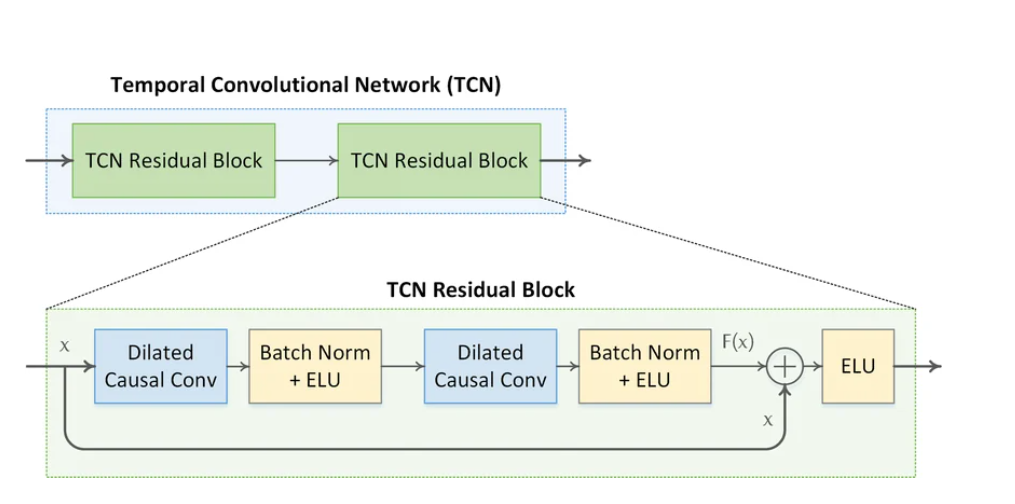
\includegraphics[width=0.8\linewidth]{image/TCN_sodo.png}
    \caption{Mô hình TCN}
    \label{fig:tcn-model}
\end{figure}

\subsubsection{Phân tích chi tiết từ hiện thực}

\begin{itemize}
    \item \textbf{Lớp TCN:} Được cấu hình với 32 bộ lọc (\texttt{nb\_filters = 32}) và kích thước nhân tích chập (\texttt{kernel\_size = 3}). Với mảng hệ số giãn cách:
    \[
    [1,\; 2,\; 4,\; 8]
    \]
    lớp này có khả năng trích xuất đặc trưng trên phạm vi thời gian rộng mà vẫn bảo toàn tính nhân quả của chuỗi dữ liệu.
    
    \item \textbf{Các lớp Dense:} Lớp ẩn với 16 nơ-ron sử dụng hàm kích hoạt ReLU giúp mô hình học được các quan hệ phi tuyến tính phức tạp giữa các thông số môi trường.
    
    \item \textbf{Kích thước mô hình:} Tổng số tham số huấn luyện là 23\,233, tương đương dung lượng khoảng 90.75 KB. Đây là kích thước rất nhỏ, phù hợp để triển khai trên Raspberry Pi 4 và đảm bảo tốc độ suy luận nhanh trong thời gian thực.
\end{itemize}

\subsection{Hiện thực Quy trình Huấn luyện và Giám sát}

Giai đoạn này tập trung vào việc hiện thực hóa quá trình huấn luyện mô hình TCN trên tập dữ liệu đã được tiền xử lý. Hệ thống được thiết kế để tự động theo dõi hiệu suất và dừng đúng thời điểm nhằm tối ưu hóa thời gian tính toán.

\subsubsection{Hiện thực cấu hình tham số huấn luyện}

Các tham số điều khiển quá trình học (\textit{hyperparameters}) được thiết lập trực tiếp trong mã nguồn \texttt{main.py} để đảm bảo tính ổn định và khả năng hội tụ của mạng nơ-ron.

\begin{itemize}
    \item \textbf{Thuật toán tối ưu (Optimizer):} Sử dụng Adam với tốc độ học (\textit{learning rate}) là $0.001$.
    
    \item \textbf{Hàm mất mát (Loss Function):} Sử dụng Mean Squared Error (MSE), đồng thời theo dõi Mean Absolute Error (MAE).
    
    \item \textbf{Kích thước lô (Batch Size):} Thiết lập bằng 32 mẫu cho mỗi lần cập nhật trọng số.
\end{itemize}

\subsubsection{Hiện thực cơ chế Giám sát và Dừng sớm (Early Stopping)}

Để ngăn chặn hiện tượng quá khớp (\textit{overfitting}) và tiết kiệm tài nguyên hệ thống, callback \texttt{EarlyStopping} được tích hợp vào quá trình huấn luyện.

\begin{lstlisting}[style=thesisstyle, language=Python]
early_stop = EarlyStopping(
    monitor='val_loss',
    patience=15,
    restore_best_weights=True
)
\end{lstlisting}

Callback này theo dõi giá trị \texttt{val\_loss}. Nếu sau 15 epoch liên tiếp không có cải thiện, quá trình huấn luyện sẽ tự động dừng và khôi phục lại bộ trọng số tốt nhất.

\subsubsection{Nhật ký thực thi quá trình huấn luyện}

Quá trình huấn luyện được khởi chạy bằng lệnh:

\begin{lstlisting}[style=thesisstyle, language=bash]
python main.py
\end{lstlisting}

Trong suốt quá trình này, hệ thống xuất ra nhật ký chi tiết cho từng epoch để theo dõi thời gian xử lý và giá trị sai số.

\begin{figure}[H]
    \centering
    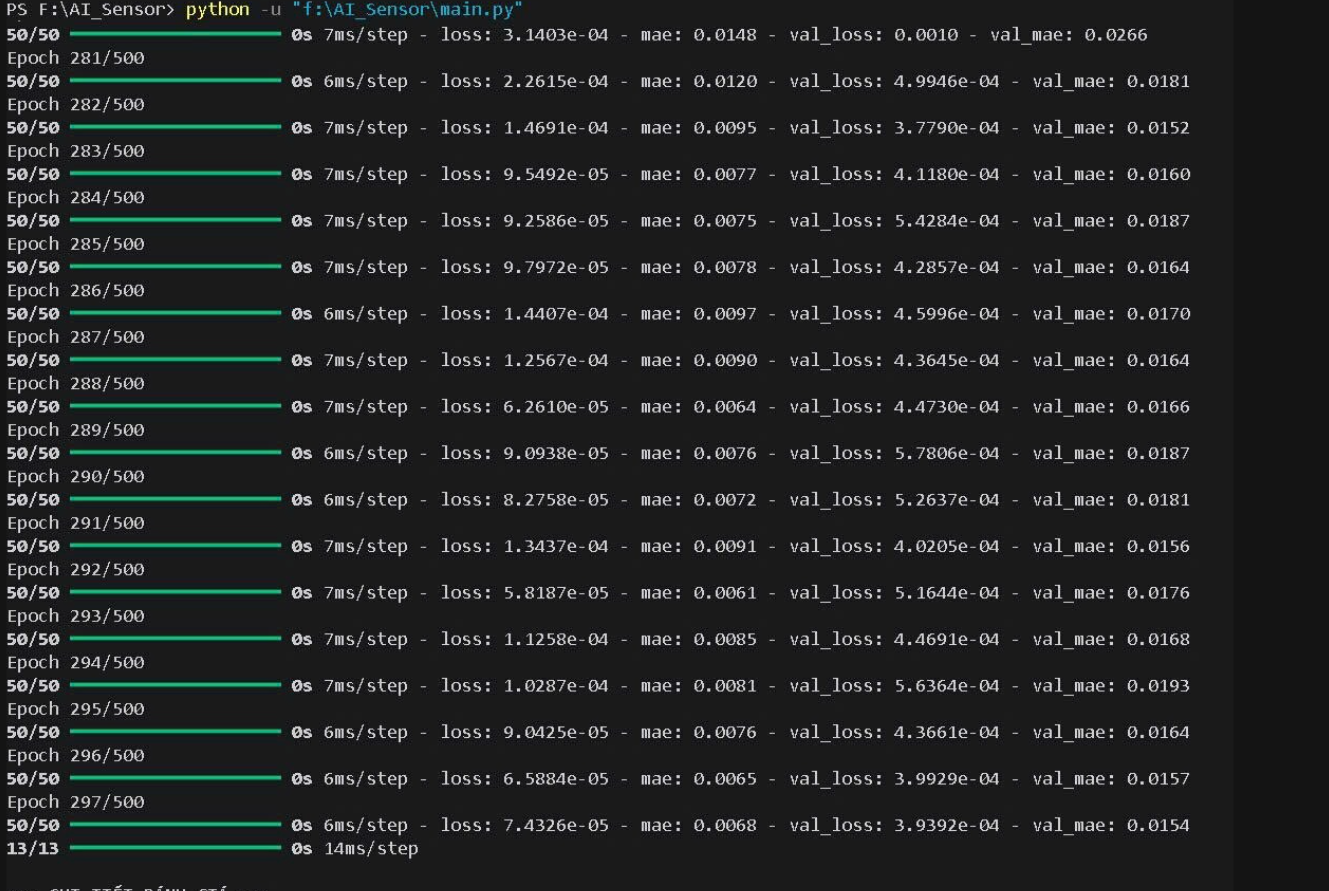
\includegraphics[width=0.7\textwidth]{image/train_quan.png}
    \caption{Nhật ký quá trình huấn luyện mô hình TCN trên môi trường máy trạm}
    \label{fig:training-log}
\end{figure}

Dựa trên nhật ký thực thi thực tế ở Hình~\ref{fig:training-log}, có thể rút ra các nhận xét sau:

\begin{itemize}
    \item \textbf{Trạng thái dừng:} Mặc dù số lượng epoch tối đa được thiết lập là 500, cơ chế Early Stopping đã tự động dừng quá trình huấn luyện tại epoch 297.
    
    \item \textbf{Hiệu suất thời gian:} Mỗi bước huấn luyện chỉ mất trung bình từ 6\,ms đến 7\,ms.
    
    \item \textbf{Đóng gói kết quả:} Sau khi huấn luyện kết thúc, mô hình được lưu vào tệp \texttt{tcn\_model.keras} để phục vụ cho bước chuyển đổi sang TensorFlow Lite.
\end{itemize}

\section{Hiện thực hệ thống cập nhập từ xa OTA}
Phần này trình bày chi tiết quá trình hiện thực hóa giải pháp cập nhật phần mềm từ xa (Over-the-Air -- OTA) cho thiết bị Raspberry Pi 4. Quá trình hiện thực bao gồm việc cấu hình môi trường build Yocto, tùy chỉnh các recipe hệ thống, xây dựng kịch bản mô tả và triển khai thực tế trên phần cứng.

\subsection{Tích hợp các Layer và Cấu hình môi trường Yocto}

Để hệ thống có khả năng xử lý OTA, bước đầu tiên là tích hợp framework SWUpdate vào quy trình xây dựng image của Yocto Project (nhánh Kirkstone).

\begin{itemize}
    \item \textbf{Quản lý Layer:} Việc tích hợp được thực hiện thông qua sửa đổi tệp \texttt{conf/bblayers.conf}. Hệ thống sử dụng layer cộng đồng \texttt{meta-swupdate} để cung cấp các công cụ lõi và layer tùy chỉnh \texttt{meta-ota} để chứa các cấu hình riêng biệt của đồ án. Cách phân tách này giúp quản lý mã nguồn dễ dàng và tránh xung đột khi cập nhật framework.

    \item \textbf{Khai báo thành phần hệ thống:} Trong tệp \texttt{conf/local.conf}, biến \texttt{IMAGE\_INSTALL:append} được khai báo để yêu cầu BitBake đóng gói các gói cần thiết vào Root File System. Các thành phần bao gồm:
    \begin{itemize}
        \item \texttt{swupdate}: chương trình chính thực hiện cập nhật.
        \item \texttt{swupdate-www}: giao diện Web UI.
        \item \texttt{libconfig}: thư viện phân tích cú pháp cho tệp \texttt{sw-description}.
        \item \texttt{u-boot-fw-utils}: công cụ giao tiếp với bootloader U-Boot.
    \end{itemize}

    \item \textbf{Tùy chỉnh Init System:} Hệ thống sử dụng \texttt{systemd} làm trình quản lý dịch vụ. Vì vậy, SWUpdate được cấu hình để hoạt động như một daemon và tự động khởi động cùng hệ thống.
\begin{lstlisting}[style=thesisstyle, language=C]
POKY_BBLAYERS_CONF_VERSION = "2"

BBPATH = "${TOPDIR}"
BBFILES ?= ""

BBLAYERS ?= " \
  /workspace/DATN-main/DATN-main/yocto/meta \
  /workspace/DATN-main/DATN-main/yocto/meta-poky \
  /workspace/DATN-main/DATN-main/yocto/meta-yocto-bsp \
  /workspace/DATN-main/layers/meta-raspberrypi \
  /workspace/DATN-main/layers/meta-openembedded/meta-oe \
  /workspace/DATN-main/layers/meta-openembedded/meta-python \
  /workspace/DATN-main/layers/meta-openembedded/meta-networking \
  /workspace/DATN-main/layers/meta-openembedded/meta-multimedia \
  /workspace/DATN-main/layers/meta-rs485 \
  /workspace/DATN-main/layers/meta-i2c \
  /workspace/DATN-main/layers/meta-qt5 \
  /workspace/DATN-main/DATN-main/yocto/build/meta-ota \
  /workspace/DATN-main/layers/meta-swupdate \
  "

\end{lstlisting}
\end{itemize}


\subsection{Hiện thực và Tùy chỉnh Recipe SWUpdate}

Hệ thống không sử dụng cấu hình mặc định mà triển khai cơ chế ghi đè (\textit{override}) thông qua tệp \texttt{swupdate\_\%.bbappend}.

\begin{itemize}
    \item \textbf{Tùy chỉnh cấu hình (Defconfig):} Thông qua lệnh:
\begin{lstlisting}[style=thesisstyle, language=bash]
bitbake swupdate -c menuconfig
\end{lstlisting}

Tùy chỉnh cấu hình (Defconfig): Thông qua lệnh bitbake swupdate -c menuconfig, hệ thống đã thực hiện tinh chỉnh các tham số quan trọng. Sau đó, tệp .config được lưu lại thành defconfig trong thư mục files của layer.

    \item \textbf{Các tùy chọn cấu hình chính:}
    \begin{itemize}
        \item \texttt{CONFIG\_LIBCONFIG=y}: Kích hoạt bộ phân tích cú pháp cho tệp \texttt{sw-description}.
        \item \texttt{CONFIG\_MONGOOSE=y}: Tích hợp máy chủ Web Mongoose vào SWUpdate để nhận gói cập nhật qua HTTP mà không cần cài thêm Nginx hoặc Apache.
        \item \texttt{CONFIG\_UBOOT=y}: Cho phép SWUpdate sử dụng thư viện \texttt{libubootenv} để ghi trực tiếp các biến môi trường của U-Boot.
    \end{itemize}

    \item \textbf{Quản lý file nguồn:} Recipe được cấu hình để bổ sung các tệp như \texttt{swupdate.service} và \texttt{hwrevision} vào thư mục \texttt{/etc/} trên Raspberry Pi 4.
\end{itemize}

    \begin{figure}[H]
    \centering
    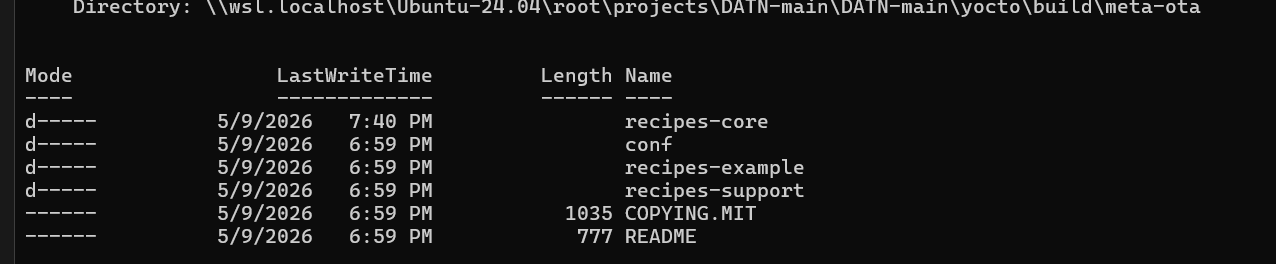
\includegraphics[width=0.7\textwidth]{image/mete-ota.png}
    \label{fig:meta-ota}
  \end{figure}
\subsection{Xây dựng Kịch bản Mô tả Hệ thống }

Tệp \texttt{sw-description} đóng vai trò là ``linh hồn'' của bản cập nhật, chứa toàn bộ thông tin định danh và chỉ thị cài đặt.

\begin{itemize}
    \item \textbf{Cấu trúc tệp:} Sử dụng định dạng Libconfig với cấu trúc phân cấp. Phần \texttt{software} định nghĩa phiên bản (ví dụ: \texttt{1.0.1}); phần \texttt{images} chứa danh sách các tệp ảnh hệ điều hành cần nạp.

    \item \textbf{Logic thực thi:} Thiết bị đích được chỉ định là \texttt{/dev/mmcblk0p3} (phân vùng dự phòng). Tham số:
\begin{lstlisting}[style=thesisstyle]
type = "raw";
\end{lstlisting}
    yêu cầu SWUpdate sử dụng cơ chế ghi dữ liệu thô theo từng sector, đảm bảo tính toàn vẹn tuyệt đối của Root File System.

    \item \textbf{Xác thực Checksum:} Mỗi mục \texttt{image} đi kèm một mã băm SHA256 để kiểm tra tính toàn vẹn dữ liệu sau khi ghi, giúp phát hiện lỗi do truyền tải mạng hoặc lỗi thiết bị lưu trữ.
\end{itemize}
\begin{lstlisting}[style=thesisstyle, language=C]
software = {
    version = "1.0.1";
    raspberrypi4-64 = {
        images: (
            {
                filename = "rootfs.ext4.gz";
                device = "/dev/mmcblk0p3"; // Phan vung dich (Slot B)
                type = "raw";
                compressed = "zlib";
                install-if-different = true;
            }
        );
        scripts: (
            {
                filename = "update_boot_env.sh";
                type = "shellscript";
            }
        );
    }
}

\end{lstlisting}
\subsection{Hiện thực Kịch bản Hậu cập nhật và Giao tiếp Bootloader}

Một trong những thách thức lớn nhất của hệ thống OTA là chuyển đổi phân vùng khởi động sau khi ghi dữ liệu thành công.

\begin{itemize}
    \item \textbf{Viết kịch bản Shell:} Hệ thống hiện thực tệp \texttt{update\_boot\_env.sh}. Tập lệnh này được SWUpdate tự động gọi sau khi quá trình ghi image hoàn tất.

    \item \textbf{Thao tác với U-Boot:} Sử dụng công cụ \texttt{fw\_setenv} để cập nhật biến môi trường của bootloader.
    \begin{itemize}
        \item \texttt{fw\_setenv ustate 1}: Đánh dấu hệ thống đang ở trạng thái cập nhật.
        \item \texttt{fw\_setenv boot\_targets mmc0:3}: Chỉ định khởi động từ phân vùng mới được cập nhật.
    \end{itemize}

    \item \textbf{Tính an toàn:} Nếu kịch bản hậu cập nhật thất bại, hệ thống sẽ không chuyển đổi slot, đảm bảo thiết bị tiếp tục khởi động vào phiên bản ổn định trước đó.
\end{itemize}

\begin{lstlisting}[style=thesisstyle, language=Python]
USTATE_INSTALLED=1
echo "--- Post-install script started ---"
echo "Setting U-Boot variable: ustate = $USTATE_INSTALLED"
fw_setenv ustate $USTATE_INSTALLED
echo "Switching boot target to Slot B..."
fw_setenv boot_slot 3
echo "--- Post-install script finished successfully ---"
exit 0
\end{lstlisting}
\subsection{Quy trình Đóng gói và Triển khai Vận hành Thực tế}

Đây là giai đoạn cuối cùng, chuyển đổi các sản phẩm từ quá trình build thành một gói cập nhật hoàn chỉnh.

\begin{itemize}
    \item \textbf{Đóng gói định dạng \texttt{.swu}:} Hệ thống sử dụng công cụ \texttt{cpio} với tùy chọn \texttt{-H crc}. Một yêu cầu bắt buộc là tệp \texttt{sw-description} phải nằm ở vị trí đầu tiên trong gói để SWUpdate có thể đọc thông tin mô tả trước khi xử lý các tệp image lớn.

    \item \textbf{Khởi chạy Daemon trên Raspberry Pi 4:}
\begin{lstlisting}[style=thesisstyle, language=bash]
swupdate -w "-r /www -p 9090"
\end{lstlisting}
    Lệnh này kích hoạt Web UI của SWUpdate tại cổng 9090.

    \item \textbf{Triển khai thực tế:} Người dùng truy cập địa chỉ IP của Raspberry Pi 4 trên cổng 9090 bằng trình duyệt. Khi tệp \texttt{.swu} được tải lên, dữ liệu sẽ được giải nén và ghi trực tiếp vào phân vùng \texttt{/dev/mmcblk0p3}. Sau khi hoàn tất, hệ thống tự động thực thi kịch bản hậu cập nhật và khởi động lại để kích hoạt phiên bản mới.
\end{itemize}

\section{Hiện thực Tool Build Yocto}

Trong quy trình phát triển hệ điều hành nhúng với Yocto Project, việc cấu hình các tệp tin \texttt{.conf} và quản lý hàng trăm lớp (\textit{layers}) metadata thường gây khó khăn và dễ dẫn đến sai sót cấu hình thủ công. Để giải quyết vấn đề này, một công cụ quản lý tập trung -- \textit{Secure-Yocto Builder} -- đã được hiện thực hóa. Công cụ này không chỉ đơn thuần là một giao diện đồ họa mà còn đóng vai trò là một lớp trung gian (\textit{Middleware}) xử lý logic nghiệp vụ, tích hợp trí tuệ nhân tạo để hỗ trợ gỡ lỗi.

\subsection{Kiến trúc phân lớp và Luồng dữ liệu}

Dựa trên sơ đồ khối hệ thống (Hình 4.5), công cụ được xây dựng theo kiến trúc 3 lớp (\textit{3-tier architecture}) nhằm đảm bảo tính module và khả năng mở rộng:

\begin{itemize}
    \item \textbf{Lớp User (Presentation Layer):} Hiện thực bằng HTML5/CSS3 và JavaScript theo phong cách Terminal User Interface (TUI). Lớp này chịu trách nhiệm thu thập thông tin cấu hình từ người dùng và hiển thị trạng thái Build theo thời gian thực.

    \item \textbf{Lớp Xử lý Logic (Business Logic Layer -- Backend):} Sử dụng framework Flask. Đây là ``bộ não'' của công cụ, thực hiện việc chuyển đổi các yêu cầu từ giao diện thành các thao tác điều chỉnh tệp tin hệ thống hoặc thực thi các lệnh Linux.

    \item \textbf{Lớp Tương tác Hệ thống (System Interaction Layer):} Bao gồm các tập lệnh Shell, công cụ BitBake của Yocto và các API bên thứ ba (Google Gemini).
\end{itemize}
\subsection{Hiện thực Lớp Backend (Flask API)}

Backend được thiết kế để xử lý các yêu cầu bất đồng bộ từ Frontend thông qua giao thức HTTP/JSON.

\subsubsection{Kỹ thuật điều khiển cấu hình bằng Biểu thức chính quy (Regex)}

Thay vì nạp toàn bộ tệp cấu hình vào bộ nhớ (có thể gây mất dữ liệu nếu tệp quá lớn), công cụ sử dụng hàm \texttt{toggle\_file\_line} để xử lý tệp tin theo từng dòng. Kỹ thuật này sử dụng Regex để tìm đúng từ khóa cấu hình và thực hiện việc comment (\texttt{\#}) hoặc uncomment dựa trên trạng thái người dùng chọn trên UI.

\begin{lstlisting}[style=thesisstyle, language=Python]
def toggle_file_line(filepath, search_pattern, enable=True):
    """
    Tu dong hoa viec cau hinh file local.conf va bblayers.conf
    """
    if not os.path.exists(filepath):
        return

    with open(filepath, 'r') as file:
        lines = file.readlines()

    with open(filepath, 'w') as file:
        for line in lines:
            # Su dung Regex de dinh vi chinh xac dong cau hinh can tac dong
            if re.search(search_pattern, line):
                if enable:
                    # Xoa ky tu comment o dau dong de kich hoat tinh nang
                    line = re.sub(r'^#\s*', '', line)
                else:
                    # Them dau comment neu nguoi dung tat tinh nang tren UI
                    if not line.startswith('#'):
                        line = f"# {line}"
            file.write(line)
\end{lstlisting}

\subsubsection{Quản lý quy trình thực thi BitBake}

Việc thực thi lệnh \texttt{bitbake} tiêu tốn rất nhiều tài nguyên và thời gian. Để tránh việc làm treo (\textit{blocking}) server Flask, công cụ sử dụng lớp \texttt{subprocess.Popen}. Toàn bộ luồng dữ liệu chuẩn (\texttt{stdout}) và luồng lỗi (\texttt{stderr}) được chuyển hướng trực tiếp ra terminal của máy chủ và đồng thời ghi vào tệp \texttt{terminal\_errors.log}.

\begin{lstlisting}[style=thesisstyle, language=Python]
@app.route('/api/start_build', methods=['POST'])
def start_build():
    # Thiet lap moi truong Yocto thong qua lenh source
    setup_env = '/workspace/DATN-main/DATN-main/yocto/oe-init-build-env'
    cmd = f"bash -c 'source {setup_env} {YOCTO_BUILD_DIR} && bitbake {image_name}' 2>&1 | tee {TERMINAL_LOG}"

    # Khoi chay tien trinh con de thuc hien build bat dong bo
    process = subprocess.Popen(
        cmd,
        shell=True,
        stdout=sys.stdout,
        stderr=sys.stderr
    )

    return jsonify({
        "status": "Success",
        "message": "Tien trinh Build da khoi dong!"
    })
\end{lstlisting}

\subsection{Hiện thực Giao diện người dùng (Frontend TUI)}

Giao diện được thiết kế để tối ưu hóa trải nghiệm cho lập trình viên hệ thống, tập trung vào sự tinh gọn và tốc độ truy cập.

\subsubsection{Quản lý trạng thái (State Management)}

Một đối tượng \texttt{state} trong JavaScript được duy trì để đồng bộ hóa các lựa chọn của người dùng (Target, Security Features, Drivers) với giao diện.

\subsubsection{Xử lý sự kiện (Event Handling)}

Khi người dùng thay đổi một tùy chọn bảo mật (như bật SELinux), một hàm \texttt{fetch} sẽ được kích hoạt để gửi tín hiệu ngay lập tức về Backend mà không cần tải lại trang.

\begin{lstlisting}[style=thesisstyle, language=Python]
async function toggleSecurityOnBackend(featureName, isChecked) {
    const featureMap = {
        'SELinux (refpolicy-mls)': 'selinux',
        'dm-verity (RootFS integrity)': 'dmverity',
        'Read-only RootFS': 'readonly'
    };

    // Gui yeu cau cap nhat file cau hinh ngay khi nguoi dung click
    await fetch('/api/toggle_security', {
        method: 'POST',
        headers: {'Content-Type': 'application/json'},
        body: JSON.stringify({
            feature: featureMap[featureName],
            value: isChecked
        })
    });
}
\end{lstlisting}

\subsection{Tích hợp các module phân tích thông minh}

\subsubsection{Module AI Debugger (Gemini Analytics)}

Khi quá trình Build gặp lỗi (\textit{Failure}), người dùng thường phải xử lý hàng nghìn dòng log phức tạp. Module \texttt{ai\_debug} được xây dựng nhằm tự động trích xuất 30 dòng lỗi cuối cùng trong tệp \texttt{terminal\_errors.log} và gửi đến mô hình Gemini 1.5 Flash để phân tích.

AI có khả năng nhận diện các lỗi phổ biến như thiếu thư viện phụ thuộc, sai cú pháp Recipe, lỗi cấu hình hoặc lỗi phân quyền truy cập. Sau khi phân tích, hệ thống sẽ trả về nguyên nhân và đề xuất hướng khắc phục bằng tiếng Việt.

Quy trình gỡ lỗi thông minh gồm các bước sau:

\begin{itemize}
    \item Trích xuất 30 dòng cuối cùng của tệp log chứa thông tin lỗi.
    \item Gửi nội dung log cùng Prompt mô tả ngữ cảnh đến Gemini 1.5 Flash.
    \item AI phân tích nguyên nhân và sinh hướng dẫn khắc phục.
    \item Kết quả được hiển thị trực tiếp trên giao diện Web.
\end{itemize}

Nhờ tích hợp AI, thời gian tìm nguyên nhân lỗi được rút ngắn đáng kể, giúp lập trình viên xử lý sự cố nhanh chóng và hiệu quả hơn.
\subsubsection{Module Quét lỗ hổng bảo mật (CVE Scan Integration)}

Đây là tính năng cốt lõi nhằm đảm bảo tính bảo mật của hệ điều hành đầu ra. Hệ thống thực thi task \texttt{cve\_check} của Yocto, sau đó Backend sẽ phân tích tệp kết quả \texttt{cve-summary.json}. Dữ liệu được phân loại theo mức độ nghiêm trọng như Critical, High và Medium, đồng thời hiển thị trực quan trên giao diện Web. Người dùng có thể nhấp vào từng mã CVE để truy cập cơ sở dữ liệu NVD (\textit{National Vulnerability Database}) và xem thông tin chi tiết.

Quy trình quét lỗ hổng được thực hiện như sau:

\begin{itemize}
    \item Yocto thực thi task \texttt{cve\_check} và sinh báo cáo \texttt{cve-summary.json}.
    \item Backend phân tích tệp JSON để trích xuất tên gói, mã CVE và mức độ nghiêm trọng.
    \item Dữ liệu được tổng hợp và hiển thị trên giao diện Web dưới dạng bảng trực quan.
    \item Người dùng có thể nhấp vào liên kết CVE để xem chi tiết trên NVD.
\end{itemize}

Tính năng này giúp lập trình viên nhanh chóng đánh giá mức độ an toàn của hệ thống và chủ động xử lý các lỗ hổng bảo mật trước khi triển khai.

